%-------------------------
% Resume in Latex
% Author : Amlaan Bhoi
% Adapted from: Sourabh Bajaj
% License : MIT
%------------------------

\documentclass[letterpaper,10pt]{article}

\usepackage{latexsym}
\usepackage[empty]{fullpage}
\usepackage{titlesec}
\usepackage{marvosym}
\usepackage[usenames,dvipsnames]{color}
\usepackage{verbatim}
\usepackage{enumitem}
\usepackage[pdftex, hidelinks]{hyperref}
\usepackage{fancyhdr}
\usepackage{pdfpages}

\usepackage[charter]{mathdesign} % Bitstream Charter
% \usepackage{newpxtext,newpxmath} % Palatino

\pagestyle{fancy}
\fancyhf{} % clear all header and footer fields
\fancyfoot{}
\renewcommand{\headrulewidth}{0pt}
\renewcommand{\footrulewidth}{0pt}

% Adjust margins
\addtolength{\oddsidemargin}{-0.50in}
\addtolength{\evensidemargin}{-0.50in}
\addtolength{\textwidth}{1in}
\addtolength{\topmargin}{-.5in}
\addtolength{\textheight}{1.0in}

\urlstyle{same}

\raggedbottom
\raggedright
\setlength{\tabcolsep}{0in}

% Sections formatting
\titleformat{\section}{
  \vspace{-6pt}\scshape\raggedright\large
}{}{0em}{}[\color{black}\titlerule \vspace{-5pt}]

%-------------------------
% Custom commands
\newcommand{\resumeItem}[2]{
  \item\small{
    \textbf{#1}{: #2 \vspace{-2pt}}
  }
}

\newcommand{\resumeItemNoBullet}[2]{
  \item[]\small{
    \hspace{-9pt}\textbf{#1}{: #2 \vspace{-6pt}}
  }
}

\newcommand{\resumeSubheading}[4]{
  \vspace{-1pt}\item[]
  \begin{tabular*}{0.98\textwidth}{l@{\extracolsep{\fill}}r}
      \hspace{-10pt}\textbf{#1} & #2 \\
      \hspace{-10pt}\textit{\small#3} & \textit{\small #4} \\
    \end{tabular*}\vspace{-5pt}
}

\newcommand{\resumeSubItem}[2]{\resumeItem{#1}{#2}\vspace{-4pt}}

\renewcommand{\labelitemii}{$\circ$}

\newcommand{\resumeSubHeadingListStart}{\begin{itemize}[leftmargin=*]}
\newcommand{\resumeSubHeadingListEnd}{\end{itemize}}
\newcommand{\resumeItemListStart}{\begin{itemize}}
\newcommand{\resumeItemListEnd}{\end{itemize}\vspace{-5pt}}

% custom commands
\newcommand{\shorterSection}[1]{\vspace{-10pt}\section{#1}}

%-------------------------------------------
%%%%%%  CV STARTS HERE  %%%%%%%%%%%%%%%%%%%%%%%%%%%%


\begin{document}

%----------HEADING-----------------
\begin{center}
  \small \textbf{{\huge Perrin Silveira}} \\  \href{mailto:perrin.silveira@pacbell.net}{\color{blue}\underline{perrin.silveira@pacbell.net}} $\vert$
  805-305-1574 $\vert$
  %LinkedIn: \href{https://www.linkedin.com/in/abhoi/}{\color{blue}\underline{abhoi}} $\vert$
  Github: \href{https://github.com/leparrain777}{\color{blue}\underline{leparrain777}} \\
  \small 527 Orchard Ave, Arroyo Grande, CA
\end{center}

%-----------EDUCATION-----------------
\shorterSection{Education}
  \resumeSubHeadingListStart
    \resumeSubheading
      {California Polytechnic State University}{San Luis Obispo, CA}
      {Bachelors of Mathematics}{March 2020}{
      \resumeItemNoBullet{Senior Project}{Deep Neural Networks and Choosing a Character in the Game Defense of the Ancients 2}
      \resumeItemNoBullet{Relevant Coursework}{Calculus Series, Linear Algebra 1 and 2, Differential Equations 1, Linear Analysis 2, Complex Analysis 1 and 2, Combinatorial Math, Theory of Numbers, Graph Theory, Mathematical Software, Discrete Math with Applications 1, Real Analysis 1 and 2, Numerical Analysis 1, Numerical Analysis 2 (Not official, lectures only), Euclidean and Modern Geometries, Abstract Algebra 1 and 2, Topology 1, Senior Project Applied Seminar, Statistical Inference/Management 1, Statistics 1, Statistical Analysis of Time Series, Mathematics Modeling Seminar(3 years), Microcontrollers for Everyone}
    }
%    \resumeSubheading
%      {Amity University}{New Delhi, India}
%      {Bachelor of Technology in Computer Science \& Engineering;  GPA: 3.32/4.0 (8.28/10.0)}{Aug 2013 - May 2017}
    %   \resumeItemNoBullet{Relevant Coursework}{Analysis \& Design of Algorithms, Data Structures using C, Operating Systems, Pattern Recognition}
  \resumeSubHeadingListEnd

%-----------SKILLS-----------------
\shorterSection{Skills}
  \resumeSubHeadingListStart
  \small
    \item{
     \textbf{Languages in order of familiarity}{: Wolfram Language (functional and symbolic manipulation),  Matlab Language (Objective C based), LaTex (document layout), Python, Java, C++, Lua }}
     \item{
     \textbf{Technologies}{: Mathematica, Matlab, Inventor, Solidworks, PrusaSlicer, AutoCAD, Github}
    }
%    \vspace{-5pt}
%    \item{
%     \textbf{Libraries}{: TensorFlow, PyTorch, Keras, Scikit-Learn, Numpy, Pandas, Spark, Jupyter, OpenCV, PIL, OpenCL, OpenGL, CUDA}
%    }
\resumeSubHeadingListEnd

%-----------EXPERIENCE-----------------
\shorterSection{Experience}
  \resumeSubHeadingListStart

    \resumeSubheading
      {California Polytechnic State University}{San Luis Obispo, CA}
      {Student}{September 2015 - March 2020}
      \resumeItemListStart
        \resumeItem{Senior Project} {Created, trained, and sourced data for a DNN to predict character choices of professional Dota 2 players}
        \begin{itemize}
            \item Created a system to pick out, format, store, and create tokenized vectors from data from Opendota.com
            \item Created both a bag-of-words neural network, and a skip-gram version of the neural network for future comparison
            \item Trained the neural network on a limited data set for testing other features
            \item Created a vector embedding for analysis of semantic similarity and vector reasoning
            \item Created a visual for the semantic similarity between characters, and using t-sne a map of relative clustering of characters to help comprehend the vector embedding
            \item Learned much more about neural networks and the theory behind them for the formal write-up, making sure I could compute a neural network out by hand instead of using pre-built codes
        \end{itemize}
          
        \resumeItem{Mathematical Software}
          {\begin{itemize}
              \item Solved hundreds of complex real-world programming problems while learning the Wolfram Language and Mathematica (can be provided upon request)
              \item Learned many of the harsh realities of programming and really began to understand the need for clear, clean, consistent, well organized, readable, and well commented code
              
          \end{itemize}
            
          }
        \resumeItem{Mathematical Modeling Seminar}
          {A class given in preparation for the Mathematical Contest in Modeling
          \begin{itemize}
              \item Year 1: Created and analyzed a model of ionospheric and ocean reflection of HF radio waves under different atmospheric conditions, and learned how to create a formal paper in LaTex for submission
              \item Year 2: Created and analyzed a model of the growth rates of the GoT dragons based upon real-world biological laws and the environmental conditions in Westeros including its extreme seasons, and created a formal paper for submission in LaTex
	   \item Year 3: Created and analyzed a model predicting vital fish migrations around Scotland under global warming scenarios examining economic impact for small fisheries and creating recommendations. Mentored two new students and established a successful team environment.
          \end{itemize}
          }
      \resumeItem{Senior Project Applied Seminar}
 	{A class targeted as a deep dive into mathematical modeling and usage of applied mathematics
          \begin{itemize}
              \item Adapted and analyzed a model of traffic flow patterns with regard to the percentage of autonomous vehicles on the road to human operated vehicles under realistic local traffic conditions.
	   \item Wrote up a full technical report, slideshow presentation, and poster for public and faculty review.
              
          \end{itemize}
          }
      \resumeItemListEnd

    \resumeSubheading
      {California Polytechnic State University}{San Luis Obispo, CA}
      {Student Researcher}{April 2019 - August 2019}
      \resumeItemListStart
       \resumeItem{Climate Research Group (Around 350-450 hrs )}
          {Dissected the papers and recreated full implementations of the climate models of Saltzman and Verbitsky in their 1992 and 1993 papers, and performed many different tasks in model validation and exploring the properties of the model itself. After implementation, specifically examined phase locking in the oscillations of the system at different levels of forcing due to solar radiation and different oscillation rates. Presented work product and poster to the public and faculty. Contact: Dr. Charles David `Dave' Camp \href{mailto:camp@calpoly.edu}{\color{blue}\underline{camp@calpoly.edu}}}
      \resumeItemListEnd

    \resumeSubheading
      {Eagle Robotics FIRST Team 1388}{Arroyo Grande, CA}
      {Student -> Mentor}{October 2011 - Present}
      \resumeItemListStart
        \resumeItem{Student (Around 170-180 hrs a year)}
          {Learned to program, fabricate, and ultimately design robots to meet various specifications of the competition
          \begin{itemize}
              \item Learned how to behave in a professional environment and how to present ideas to other team members and the public at events
              \item Learned how to work safely and efficiently to construct parts to specification in a machine shop
              \item Learned how to how to design optimally and operate different design softwares (Autodesk Inventor and AutoCAD) independently during the summer so that I could take on a lead design role my senior year
          \end{itemize}
          }
          \resumeItem{Mentor (Around 150-170 hrs a year)}
          {Taught and assisted students in the process of designing and building a robot
          \begin{itemize}
              \item Learned a new design software (Solidworks) so that I could help the students with the problems they encountered in the design process
              \item Supervised and helped instruct students and other mentors on the operation of various tools in the machine shop including milling, lathe operation, and tig welding
              \item Created an independent and mathematical implementation of swerve drive, a more complicated drive terrain style, in Mathematica and implemented the model constructed in the Java framework the robot is controlled with. Became much more familiar working in an object-oriented language. Project public on GitHub. Disclaimer: I had no instruction on coding style for object-oriented languages and no code reviews or testing has been done due to Covid-19.
	   \item Independently developed the skills and knowledge base to be able to successfully 3D-print a large variety of 3D models so that as a team we could both continue teaching students how to operate a 3D-printer, and integrate 3D-printing into our design process. Previously, 3D-printing had been a student-led project of which all students suddenly left the team, and our printer only got used by our public relations subteam as a means to advertise due to reliability issues.
          \end{itemize}
          }
      \resumeItemListEnd

  \resumeSubHeadingListEnd

%-----------PROJECTS-----------------
\shorterSection{Side Projects / Activities}
  \resumeSubHeadingListStart
    \resumeSubItem{Continuation of Senior Project}
     {My current hope is to expand my project to run as a website that automatically fetches data, trains, and displays the output of the neural network and vector embeddings. Also included would be a small analytic engine using the properties of the vector embedding for computations on character vectors. 
%        \vspace{-5pt}
%        \begin{itemize}
%            \item Implemented a CRF in $O(m|\mathcal{Y}|^2)$ time to achieve a 84\% letter-wise accuracy on UPenn OCR dataset
%            \item Implemented OpenMPI CRF using PETSc and Tao to achieve 77.1\% letter-wise accuracy
%        \end{itemize}
     }
    \resumeSubItem{An actually useful music visualizer}{Incomplete: Creation of a music visualizer that uses mode decomposition to wrap the approximate amplitude of the notes being played around a circle in such a way that the different octaves of the same note will stack additively where each octave layer will have a different color. This is so a musician could easily pull out the notes being played in a song along with the octave without having to consult a spectrogram and a chart of note frequencies.}
    \resumeSubItem{Dota 2 Modding}
      {Created a script that generates a complete text file organizing key-value pairs that are randomized within certain bounds for a Dota 2 custom game mode. Ongoing: Learning Lua scripting using Dota specific documentation and other users GitHub projects to create multiple of my own custom game modes.}
    \resumeSubItem{Marching Band Volunteer Instructor}
      {Mentored and helped train students in proper marching form, and strength and endurance building. Also served as the main equipment transporter and sound tech during practices and performances. Two years of ~80 hours for band camp, and ~10 hrs a week for the following 3 months or so }
    \resumeSubItem{Volunteer Fireworks Salesman}
      {Served 3+ years as a fireworks salesman for the local band and the local robotics team on years they are selected to have a booth. Roughly 6-6.5 hours every day for a week once a year helping customers find the perfect composition of fireworks to fit their needs and their budget.}
%    \resumeSubItem{AI Lifeguard}{Trained a 3D-CNN model on Microsoft Azure for action localization on drowning people in %swimming pools. Achieved mean IOU score of 0.45}
  \resumeSubHeadingListEnd

%-----------Addtional Experience & Achievements-----------------
%\shorterSection{Additional Experience \& Achievements}
%  \resumeSubHeadingListStart
%  \small
%    \item{Presented poster on \textit{Tiramisu DenseNet Architecture for Precise Segmentation} for Intel AI at \textbf{CVPR %2018}}
%    \vspace{-5pt}
%    \item{Selected as an \textbf{Intel AI Student Ambassador} (only 150 students) to research, publish, and share work on %machine learning and deep learning}
%    \vspace{-5pt}
%    \item{Won \textit{Best Microsoft Hack} out of 220 teams at \textbf{HackHarvard 2017}}
%    \vspace{-5pt}
%    \item{Placed 16/50 at Google Games: Campus Edition 2017 at UIC}
%    \vspace{-5pt}
%    \item{Won \textit{Best Technical Innovation} award (out of 800 students) at \textbf{Amity University Convocation 2017}}
%    \vspace{-5pt}
%    \item{Elected as a \textit{Vice-Chair} for \textbf{ACM Amity Student Chapter} out of 800 students at Amity University %based on high-achieving and technically strong undergraduate students}
%  \resumeSubHeadingListEnd
%-------------------------------------------
%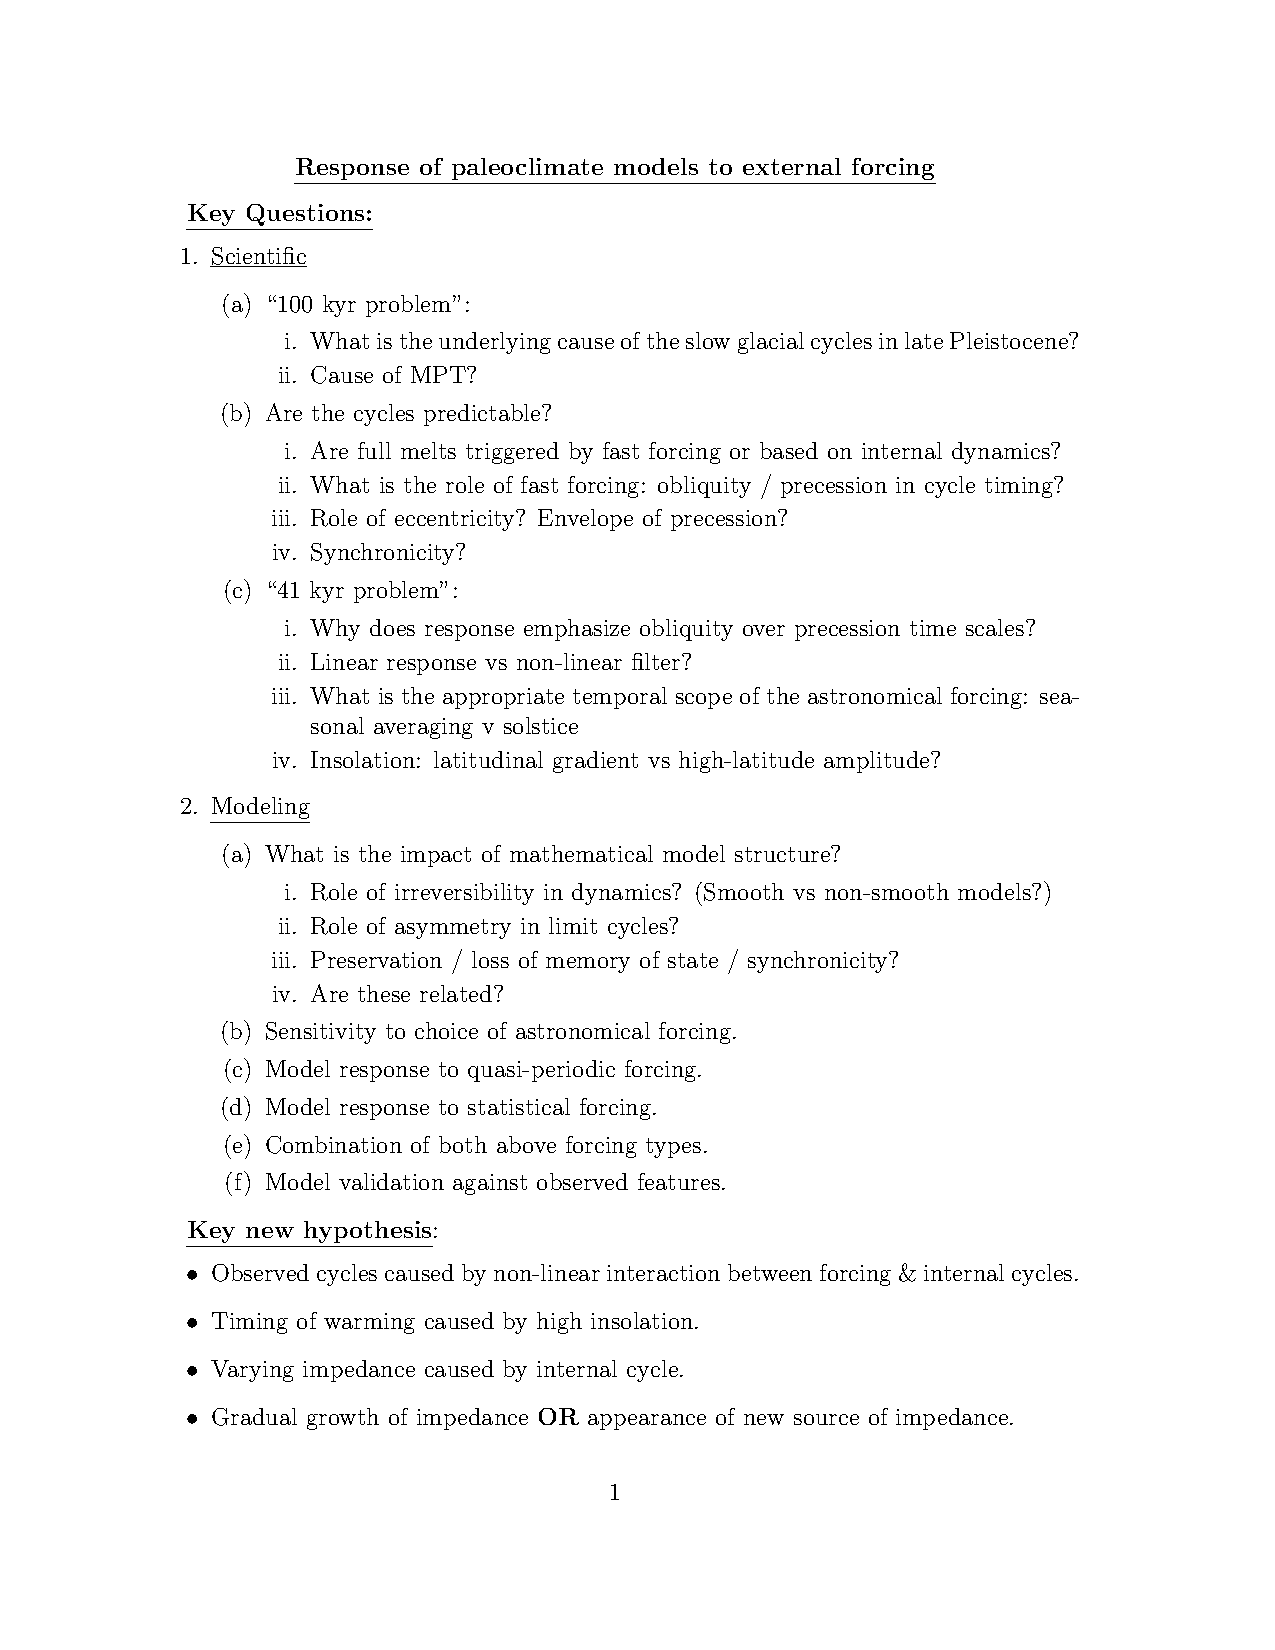
\includepdf[pages=-]{ResearchSummary_SQ19.pdf}
\end{document}
